\documentclass[10pt,a4paper]{article}
\usepackage[utf8]{inputenc}
\usepackage[T1]{fontenc}
\usepackage{fullpage}
\usepackage{amsfonts,amsmath,amssymb,mathtools, bm}
\usepackage{comment,color, fancybox}
\usepackage{verbatim}
\usepackage{enumitem}
\usepackage{listings}
\usepackage{xcolor}
\usepackage{array}
\usepackage{ragged2e}
\usepackage{csvsimple}
\usepackage{changepage}
% \usepackage[alf]{ABNTex/abntex2cite}
\usepackage[ddmmyyyy]{datetime}

\lstset{language=C++,
	basicstyle=\ttfamily,
	keywordstyle=\color{blue}\ttfamily,
	stringstyle=\color{green}\ttfamily,
	commentstyle=\color{gray}\ttfamily,
	morecomment=[l][\color{magenta}]{\#}
}

\newcommand{\ttt}[1]{\texttt{#1}}

\title{Relatório do Desempenho de Aplicações Paralelas Usando OpenMP} 
\author{Miguel Nunes}
\date{\today}

\begin{document}
	\maketitle

	\section{Algoritmos e Descrição do Ambiente}

		Foi analisado o algoritmos de Mandelbrot paralelizado usando \textit{pthreads} e Open MP, 
		com apenas leves modificações na entrada de dados e alocação de memória para facilitar a automatização dos testes.
		Foram utilizadas os valores como entrada: 
		
		\begin{verbatim}
			max_row    = 340
			max_column = 1000
			max_n      = 4600
		\end{verbatim}

		Pois foi observado experimentalmente que, em execuções sequenciais do algoritmo, essas entradas levavam, em média, 
		64 segundos para serem processadas.

		Os testes foram realizados num computador com as seguintes especificações:

		\begin{description}
			\item[CPU] \texttt{AMD Ryzen 7 5700G with Radeon Graphics (16) @ 4.673GH}
			\item[Memória] \texttt{63588MiB}
			\item[OS] \texttt{Fedora Linux 36 (MATE-Compiz) x86\_64}
			\item[Kernel] \texttt{5.18.19-200.fc36.x86\_64}
		\end{description}

		Os testes foram executados automaticamente a partir de um script em bash, com o auxílio de um makefile. As entradas para os 
		testes eram geradas pelo makefile, ao início de uma nova rodada de testes, todos os arquivos gerados no teste anterior são deletados.

		Apenas foi testada a versão do algoritmo em Open MP, já que a versão com \textit{pthreads} havia sido testada no trabalho anterior.

	\section{Coleta dos Dados}
		
		Ao fim da execução dos algoritmos, o tempo levado para realizar seu cálculo e a quantidade de \textit{threads} utilizada é
		é imprimida para \texttt{stdout}. Nos testes \texttt{stdout} era redirecionado para um arquivo de texto por meio de 
		operações de \textit{pipe} do bash. O nome dos arquivos de saída segue o formato \break \texttt{algoritmo\_númeroTeste\_númeroThreads}, 
		onde \_ é apenas um separador para visualização e não estava de fato no nome dos arquivos.
		Por exemplo, o arquivo \texttt{mandelbrotStatic16} se refere a segunda execução do algoritmo de mandelbrot com 6 \textit{threads} usando
		o \textit{schedule} estático.

		Foi feito um script em \textit{Python} versão 3.10 para processar esses dados. Os arquivos são lidos ``em massa'' e seus dados são carregados em
		estruturas \textit{dict} para serem manipulados. Os dados obtidos são os seguintes:

		\begin{table}[htb]
			\begin{adjustwidth}{-1cm}{}
				\csvautotabular{mandelbrot.csv}
				\caption{Dados da execução do algoritmo de Mandelbrot com \textit{pthreads}}
			\end{adjustwidth}
		\end{table}
		\begin{table}[htb]
			\begin{adjustwidth}{-1cm}{}
				\csvautotabular{static.csv}
				\caption{Dados da execução do algoritmo de Mandelbrot com \textit{schedule} estático}
			\end{adjustwidth}
		\end{table}
		\begin{table}[htb]
			\begin{adjustwidth}{-1cm}{}
				\csvautotabular{dynamic.csv}
				\caption{Dados da execução do algoritmo de Mandelbrot com \textit{schedule} dinâmico}
			\end{adjustwidth}
		\end{table}
		\begin{table}[htb]
			\begin{adjustwidth}{-1cm}{}
				\csvautotabular{guided.csv}
				\caption{Dados da execução do algoritmo de Mandelbrot com \textit{schedule} guiado}
			\end{adjustwidth}
		\end{table}

	\clearpage
	\section{Análise do Dados}

		Sobre os dados apresentados acima, podemos obter as seguintes informações, onde o tempo é medido em segundos:

		\begin{table}[htb]
			\begin{tabular}{|c|c|c|}
				\hline
				& Média do Tempo de Execução & Desvio Padrão\\ \hline
				1 Thread  & 64.777607 & 0.16630814071409003 \\ \hline
				2 Threads & 32.897305 & 0.16732219181035715 \\ \hline
				3 Threads & 40.482982 & 0.04887138853948963 \\ \hline
				4 Threads & 27.345909 & 0.10432392396335134 \\ \hline
				5 Threads & 27.095582 & 0.05337008271390313 \\ \hline
				6 Threads & 20.748611 & 0.04259400204254115 \\ \hline
				7 Threads & 19.685831 & 0.03082819193170025 \\ \hline
				8 Threads & 16.775065 & 0.02461598543404037 \\ \hline
			\end{tabular}
			\caption{Médias e desvio padrão do algoritmo de Mandelbrot com \textit{pthreads}}
		\end{table}

		\begin{table}[htb]
			\begin{tabular}{|c|c|c|}
				\hline
				& Média do Tempo de Execução & Desvio Padrão \\ \hline
				1 Thread  & 9.808757 & 0.01430773997993158 \\ \hline
				2 Threads & 4.975305 & 0.02110255184674231 \\ \hline
				3 Threads & 6.125578 & 0.01186485735270328 \\ \hline
				4 Threads & 4.136371 & 0.01319911566903059 \\ \hline
				5 Threads & 4.088702 & 0.00786163087406173 \\ \hline
				6 Threads & 3.127701 & 0.00801616623524678 \\ \hline
				7 Threads & 3.027129 & 0.01203302441893417 \\ \hline
				8 Threads & 2.565438 & 0.00671966070572017 \\ \hline
			\end{tabular}
			\caption{Médias e desvio padrão do algoritmo de Mandelbrot com \textit{schedule} estático}
		\end{table}

		\begin{table}[htb]
			\begin{tabular}{|c|c|c|}
				\hline
				& Média do Tempo de Execução & Desvio Padrão \\ \hline
				1 Thread  & 9.818728 & 0.01456274836698083 \\ \hline
				2 Threads & 4.976967 & 0.01513441336087318 \\ \hline
				3 Threads & 6.124495 & 0.01606536734026911 \\ \hline
				4 Threads & 4.130273 & 0.01311360790256527 \\ \hline
				5 Threads & 4.095747 & 0.00969797579108356 \\ \hline
				6 Threads & 3.124399 & 0.01151921626384943 \\ \hline
				7 Threads & 3.028609 & 0.00966705286584861 \\ \hline
				8 Threads & 2.559377 & 0.00553523019695965 \\ \hline
			\end{tabular}
			\caption{Médias e desvio padrão do algoritmo de Mandelbrot com \textit{schedule} dinâmico}
		\end{table}

		\begin{table}[htb]
			\begin{tabular}{|c|c|c|}
				\hline
				& Média do Tempo de Execução & Desvio Padrão \\ \hline
				1 Thread  & 9.812667 & 0.01803282319056608 \\ \hline
				2 Threads & 4.974860 & 0.014412573985547702 \\ \hline
				3 Threads & 6.127850 & 0.010964194452854417 \\ \hline
				4 Threads & 4.133592 & 0.01210745298474367 \\ \hline
				5 Threads & 4.092610 & 0.008310102285772432 \\ \hline
				6 Threads & 3.126775 & 0.00917122098983795 \\ \hline
				7 Threads & 3.024289 & 0.009009298221528924 \\ \hline
				8 Threads & 2.565941 & 0.006704982310027237 \\ \hline
			\end{tabular}
			\caption{Médias e desvio padrão do algoritmo de Mandelbrot com \textit{schedule} guiado}
		\end{table}
		
		É evidente que o aumento de threads diminui significativamente o tempo de execução dos algoritmos sem causar 
		aumento significativo no desvio padrão, assim como que a utilização do Open MP, mesmo nos casos com apenas 1 thread, significativamente diminui o tempo
		de execução do algoritmo, como pode ser observado no gráfico abaixo, onde as execuções [0,\ldots,9] tem 1 thread, as execuções [10,\ldots,19] tem duas threads
		e assim por diante:
		
		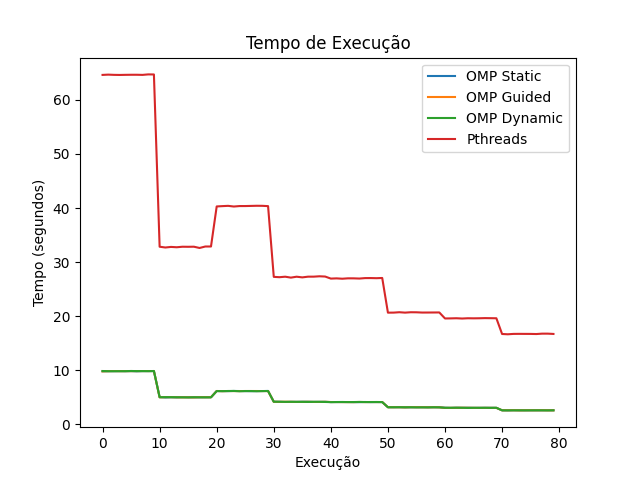
\includegraphics[scale=.7]{TempoExecução.png}
		
		Ademais, os seguinte gráficos de aceleração e eficiência foram elaborados:
		
		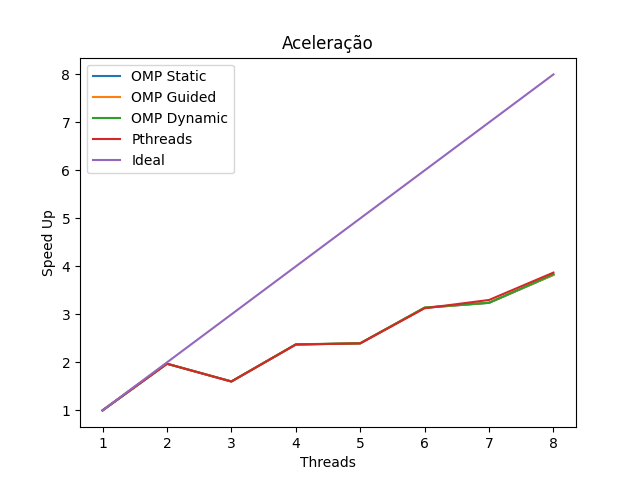
\includegraphics[scale=.7]{Aceleração.png}
		\clearpage

		É possível observar que o algoritmo de Mandelbrot com \textit{pthreads} não teve bom desempenho ao ser paralelizado, apesar de 
		ter um aumento de performance significativo em uma execução com 8 threads se comparada com a execução sequencial, 
		esse aumento não é tão grande se comparado com uma execução com apenas 6 threads. Mais ainda, o desempenho não é consistente, isto é,
		houveram situações onde execuções com menos threads tiveram desempenho melhor que execuções com mais threads.

		Isso também ocorre, porém de maneira menos significativa nos casos de uso do Open MP, onde, apesar do tempo absoluto ser significativamente
		menor que nos casos de \textit{pthreads}, as taxas de aceleração se mantiveram as mesmas.

		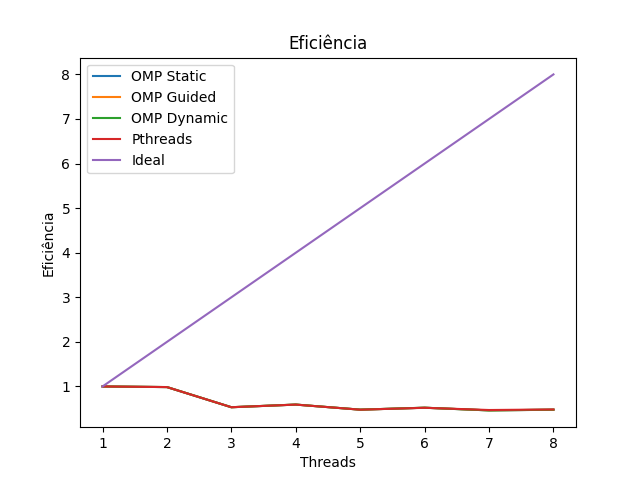
\includegraphics[scale=.7]{Eficiência.png}
		
		O algoritmo de Mandelbrot com \textit{pthreads} novamente teve um desempenho ruim. O gráfico torna evidente
		que este algoritmo, na sua implementação testada, não lida bem com paralelização além de duas threads.
		A baixa eficiência do algoritmo nos casos com mais de duas threads pode ser interpretada como uma indicação que
		a implementação de paralelismo testada não é a ideal e pode ser melhorada.

		O mesmo pode ser dito para os casos de uso de Open MP, e específico a estes, o uso de diferentes \textit{schedules} de paralelismo não
		tiverem impacto significativo nas taxas de aceleração ou eficiência do algoritmo.

\end{document}